\documentclass{article}
\usepackage[T2A]{fontenc}
\usepackage{epigraph}
\usepackage[english, russian]{babel} % языковой пакет
\usepackage{amsmath,amsfonts,amssymb} %математика
\usepackage{mathtools}
\usepackage[oglav,spisok,boldsect,eqwhole,figwhole,hyperref,hyperprint,remarks,greekit]{../../style/fn2kursstyle}
\usepackage[utf8]{inputenc}
\usepackage[]{tkz-euclide}
\usepackage{algpseudocode}
\usepackage{pgfplots}
\usepackage{tikz-3dplot}
\usepackage[oglav,spisok,boldsect,eqwhole,figwhole,hyperref,hyperprint,remarks,greekit]{./style/fn2kursstyle}
\usepackage{multirow}
\usepackage{supertabular}
\usepackage{multicol}
\usepackage{tikz}
\usepackage{pgfplots}
\usepackage{float}
\usepackage{graphicx}
\pgfplotsset{compat=1.9}
\usepackage[svgnames]{pstricks}
\usepackage{pst-solides3d} 
\usepackage{multirow}
\usepackage{hhline}
\usepackage{slashbox}
\usepackage{pdflscape}
\usepackage{array} 
\graphicspath{{../../style/}}
  



\newcommand{\cond}{\mathop{\mathrm{cond}}\nolimits}
\newcommand{\rank}{\mathop{\mathrm{rank}}\nolimits}
% Переопределение команды \vec, чтобы векторы печатались полужирным курсивом
\renewcommand{\vec}[1]{\text{\mathversion{bold}${#1}$}}%{\bi{#1}}
\newcommand\thh[1]{\text{\mathversion{bold}${#1}$}}
%Переопределение команды нумерации перечней: точки заменяются на скобки
\renewcommand{\labelenumi}{\theenumi)}
\newtheorem{theorem}{Теорема}
\newtheorem{define}{Определение}
\tdplotsetmaincoords{60}{115}
\pgfplotsset{compat=newest}

\title{Итерационные методы решения систем
линейных алгебраических уравнений}
\author{Н.\,О.~Акиньшин}
\group{ФН2-51Б}
\date{2024}
\supervisor{А.\,С.~Джагарян}



\begin{document}
    \maketitle
    \newpage
    \tableofcontents
    \newpage

    \section{Контрольные вопросы}
    \begin{enumerate}
        \item Почему условие $\|C\| < 1$ гарантирует сходимость итерационных методов?
        \newline
        {\bfseries Ответ.}
        Любой одношаговый итерационный метод можно записать в виде 
        \begin{equation*}
            B_{k+1}\frac{x^{k+1} - x^k}{\tau_{k+1}} + A x^k = b, \ k = 0, 1, 2,\ldots
        \end{equation*}
        Из этого вида можно прийти к следующему:
        \begin{equation}
            x^{k+1} = Cx^k + y
            \label{special form iter method}
        \end{equation}
        Подставив истинное решение $x$ в~\eqref{special form iter method},
        получим 
        \begin{equation*}
            x \equiv  Cx + y 
        \end{equation*}
        Тогда, вычитая из~\eqref{special form iter method},
        \begin{equation*}
            x^{k+1} - x = C(x^{k} - x)
        \end{equation*}
        Переходя к выражению с нормами
        \begin{equation*}
            \|x^{k+1} - x\| = \|C(x^{k} - x)\| \leqslant
           \|C\| \|x^{k} - x\| \leqslant \ldots \leqslant \|C\|^{k}\|x_0 - x\|
        \end{equation*}
        Если $\|C\| < 1$, то последовательность сходится $\{x^k\}_{k=1}^\infty$ сходится к $x$ для 
        любого $x_0$.

        
        \item Каким следует выбирать итерационный параметр $\tau$ в методе 
        простой итерации для увеличения скорости сходимости?
        Как выбрать начальное приближение $x_0$?
        \newline
        {\bfseries Ответ.}
        Пусть $x$-истинное решение системы $Ax=f$. Метод простой итерации можно представить в виде $\frac{x^{k+1}-x^k}{\tau}+Ax^k=f$, где $x^k$--koе приближение истинного решения. Введем обозначение $z^k=x^k-x$--погрешность. Тогда метод простой итерации можно переписать $\frac{z^{k+1}-z^k}{\tau}+Az^k=0$. Отсюда $z^{k+1}=(E + \tau A) z^k$. Перейдем к норме
	\[
	||z^{k+1}||\le||(E + \tau A)|| \cdot ||z^k||\le ||(E + \tau A)||^{k+1} \cdot ||z^0|| =||(E + \tau A)||^{k+1} \cdot ||x^0-x||
	\]
	Из данного соотношения можно сделать вывод, что параметр $\tau$ нужно выбрать так чтобы норма матрицы $(E+\tau A)$ была как можно меньше, а начальное приближение выбрать как можно ближе к истинному решению.

        \item На примере системы из двух уравнений с двумя неизвестными
        дайте геометрическую интерпретацию метода метода
        Якоби, метода Зейделя, метода релаксации.
        \newline
        {\bfseries Ответ.}
        Рассмотрим метод Якоби.
        \begin{equation}
            \begin{dcases}
                a_{11}x_1^{k+1} + a_{12}x_2^k = b_1, \\
                a_{21}x_1^{k} + a_{22}x_2^{k+1} = b_2,
            \end{dcases}
            \label{system_jacoby}
        \end{equation}
        Пусть $l_1: a_{11}x_1^{k+1} + a_{12}x_2^k = b_1$, и 
        $l_2: a_{21}x_1^{k} + a_{22}x_2^{k+1} = b_2$ -- прямые, задаваемые уравнениями системы.
        Точка их пересечения и есть истинное решение системы~\eqref{system_jacoby}. 
        На рис.~\ref{jacoby_graph} видно, что с каждой итерацией точка $x^k = (x_1^k, x_2^k)$ 
        сходится к истинному решению $x$, причем каждая точка $x^k$ лежит внутри области, ограниченных прямыми.
        Причем ни одна из итеративных точек не лежит на прямых.
        \begin{figure}[H]
            \center
            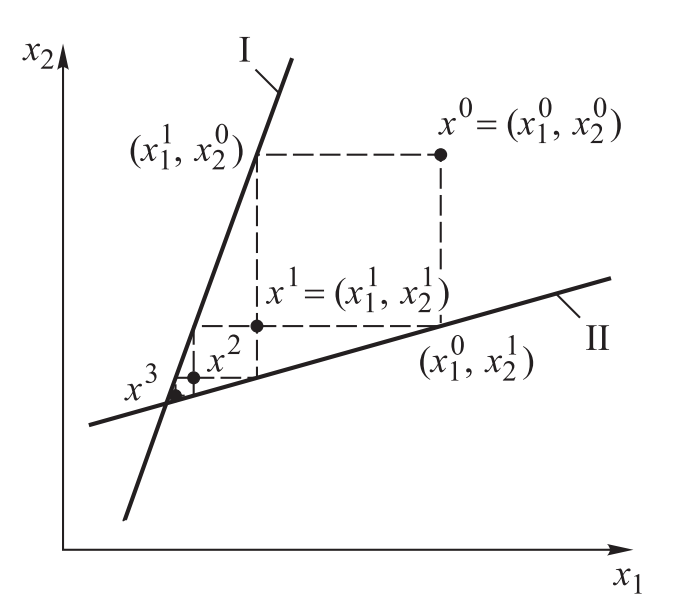
\includegraphics[width=0.5\textwidth]{jacoby_graph.png}
            \caption{Графический смысл метода Якоби}
            \label{jacoby_graph}
        \end{figure}
        Рассмотрим метод Зейделя.
        \begin{equation}
            \begin{dcases}
                a_{11}x_1^{k+1} + a_{12}x_2^k = b_1, \\
                a_{21}x_1^{k+1} + a_{22}x_2^{k+1} = b_2,
            \end{dcases}
            \label{system_seidel}
        \end{equation}
        Аналогично, принимая за прямые $l_1 = a_{11}x_1^{k+1} + a_{12}x_2^k = b_1$ и 
        $l_2 = a_{21}x_1^{k+1} + a_{22}x_2^{k+1} = b_2$ за прямые. Изобразим эти прямые на 
        рис.~\ref{seidel_graph}. Из рис.~\ref{seidel_graph} видно, что все точки лежат на прямых.
        \begin{figure}[H]
            \center
            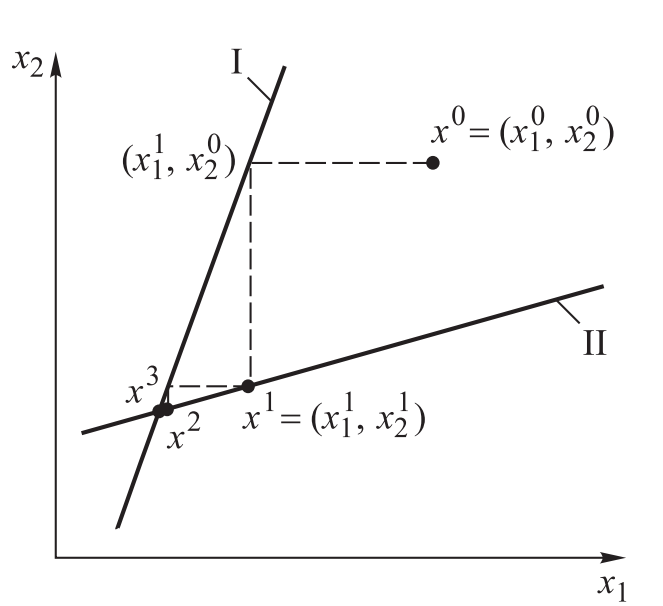
\includegraphics[width=0.5\textwidth]{seidel_graph.png}
            \caption{Графический смысл метода Зейделя}
            \label{seidel_graph}
        \end{figure}

        Рассмотрим метод релаксации. 
        \begin{equation}
            \begin{dcases}
                a_{11} (x_1^{k+1} - x_1^k) = \omega (-a_{11}x_1^k - a_{12}x_2^k +f_1), \\ 
                a_{22} (x_2^{k+1} - x_2^k) = \omega (-a_{21}x_1^k - a_{22}x_2^k +f_2)
            \end{dcases}
        \end{equation}
        Пусть $\boldsymbol{l_1} = (a_{11}, -a_{12})$ -- вектор нормали первой прямой, тогда 
        величина 
        \begin{equation*}
        |\omega (-a_{11}x_1^k - a_{12}x_2^k +f_1)| = \omega d_1 \|\boldsymbol{l_1}\|,
        \end{equation*}
        где $d_1$ -- расстояние от $(x_1^k, x_2^k)$ до первой прямой.
        При этом направление смещения вдоль оси
        абсцисс определяется тем, в положительной или отрицательной
        полуплоскости относительно прямой I расположена точка $(x_1^k, x_2^k)$.
        Заметим, что 
        \begin{equation*}
            |x_1^{k+1} - x_1^k| = \omega \dfrac{d_1}{|a_{11} / \|\boldsymbol{l_1}\||} = 
            \omega \dfrac{d_1}{|\cos \beta_1|},
        \end{equation*}
        где $\beta_1$ -- угол между первой прямой и осью координат.

        \begin{figure}[H]
            \center
            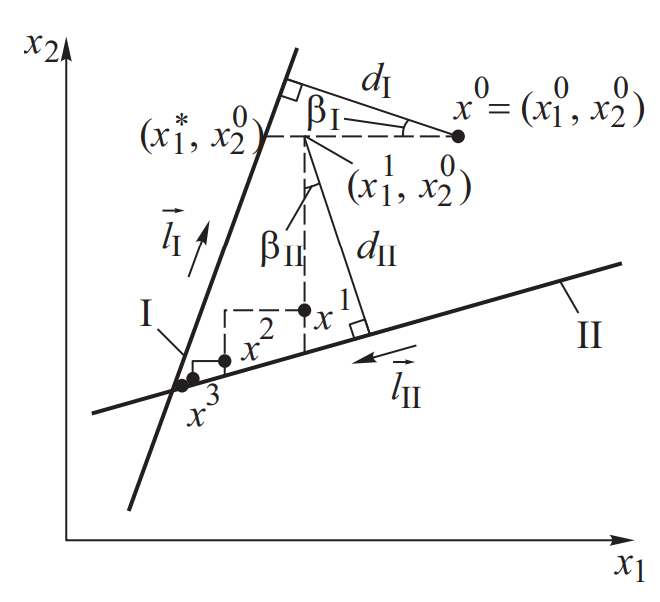
\includegraphics[width=0.5\textwidth]{lower_relaxation.png}
            \caption{Графический смысл метода релаксации при $\omega < 1$}
            \label{lower_relax_graph}
        \end{figure}

        \begin{figure}[H]
            \center
            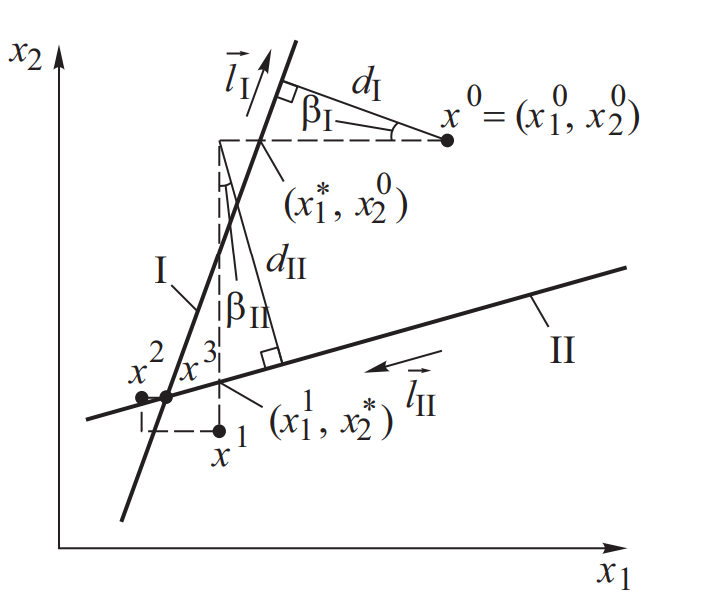
\includegraphics[width=0.5\textwidth]{upper_relaxation.png}
            \caption{Графический смысл метода релаксации при $\omega > 1$}
            \label{upper_relax_graph}
        \end{figure}

        \item При каких условиях сходятся метод простой итерации,
        метод Якоби, метод Зейделя и метод релаксации? Какую
        матрицу называют положительно определенной?
        \newline
        {\bfseries Ответ.}
        \textbf{Определение} Матрица $A$ называется положительно определенной $A>0$, если $\forall x \, (Ax, x) > 0 $.
	
	
	\noindent Рассмотрим теорему о сходимости стационарного итерационного метода.
	
	\textbf{Теорема} Пусть $A--$ симметричная положительно определенная матрица, $\tau > 0$ и выполнено неравенство 
	\[
	B-0.5\tau A
	\]
	Тогда стационарный итерационный метод 
	\[
	B\frac{x^{k+1}-x^k}{\tau} + Ax^k = f
	\]
	сходится при любом начальном приближении $x^0$.
	
	
	\textbf{Доказательство} Пусть $x^k=x^k-x$--погрешность k--й итерации. Поскольку $f=Ax$, то 
	\[
	B\frac{z^{k+1}-z^k}{\tau} + Az^k = 0
	\]
	Необходимо показать,что норма погрешности стремится к нулю при $k \rightarrow \infty$. Проведем преобразования:
	\[
	z^{k+1}=(E-\tau B^{-1}A)z^k
	\]
	\[
	Az^{k+1}=(A-\tau AB^{-1}A)z^k
	\]
	\[
	(Az^{k+1},z^{k+1})= ((A-\tau AB^{-1}A)z^k, (E-\tau B^{-1}A)z^k)=
	\]
	\[
	(Az^k,z^k)-\tau (Az^k,B^{-1}Az^k) - \tau (AB^{-1}Az^k,z^k) + \tau^2(AB^{-1}Az^k,B^{-1}Az^k).
	\]
	В силу симметрии A имеем 
	\[
	(AB^{-1}Az^k,z^k) = (B^{-1}Az^k, Az^k)
	\]
	Следовательно,
	\[
	J_{k+1}=(Az^{k+1},z^{k+1}) = J_{k} - 2 \tau ((B-0.5 \tau A)B^{-1}Az^k,B^{-1}Az^k) + \tau^2(AB^{-1}Az^k,B^{-1}Az^k)
	\]
	
	
	Если $B-0.5\tau A>0$, то $J_{k+1}\le J_{k}, J_{k} \ge 0$, так как $A>0$. Отсюда заключаем, что последовательность $J_k$ монотонно не возрастает и ограничена нулем снизу. Поэтому существует предел последовательности:

        \item Выпишите матрицу $C$ для методов Зейделя и релаксации.
        \newline
        {\bfseries Ответ.} 
        Рассмотрим метод Зейделя.
        Будем считать, что $A = L + D + U$, где $L$ -- нижнетреугольная матрица, $D$ -- 
        диагональная матрица, $U$ -- верхнетреугольная матрица.
        Тогда метод Зейделя можно представить в каноническом виде: 
        \begin{equation*}
            (D + L)(x^{k+1} -x^k) + Ax^k = f
        \end{equation*}
        Из этого вида получаем:
        \begin{equation*}
            C = E - (D+L)^{-1}A
        \end{equation*}

        Рассмотрим метод релаксации.
        Метод релаксации можно представить в каноническом виде: 
        \begin{equation*}
            (D + \omega L)\frac{x^{k+1} -x^k}{\omega} + Ax^k = f
        \end{equation*}
        Тогда 
        \begin{equation*}
            C = E - \omega(D+\omega L)^{-1}A
        \end{equation*}
        \item Почему в общем случае для остановки итерационного
        процесса нельзя использовать критерий $\|x^k - x^{k+1}\| < \varepsilon$?
        \newline
        {\bfseries Ответ.}
        Алгоритм может получить такие значения $x_k$, что 
        $\|x^k - x^{k+1}\| < \varepsilon$, но при этом $x_k$ будет далеко от $x^*$.
        Приведем пример: 
        
        \item Какие еще критерии окончания итерационного процесса
        Вы можете предложить?
        \newline
        {\bfseries Ответ.}

        Рассмотрим критерий останова $\|x^{k+1} - x^k\| < \varepsilon$. Его достоинством
        можно считать простоту вычисления, однако он обладает существенным недостатком. Если 
        алгоритм уменьшает скорость схождения, но при этом не сходится к истинному решению, то данный 
        критерий вынудит алгоритм остановиться, а также не отражает связи между истинным решением и полученным: 
        \begin{equation*}
            \|x^{k+1} - x^k \| = \|x^{k+1} - x + x - x^k\| \leqslant \|x^{k+1} - x\| + \|x^k - x\| \not \leqslant \varepsilon   
        \end{equation*}

        Рассмотрим критерий останова 
        $\dfrac{\|x^{k+1} - x^k\| }{\|x^k\|+ \varepsilon_0} < \varepsilon$.
        Его достоинством по сравнению с предыдущем критерием является то, что 
        он вычисляет разность между решениями относительно предыдущего решения, то есть 
        он может заставить алгоритм остановиться только тогда, когда относительная скорость 
        схождения будет достаточно малой, в отличие от абсолютной, как это указано в предыдущем критерии.
        Недостатком можно считать наличие двух параметров $\varepsilon_0, \ \varepsilon$.

        Рассмотрим критерий останова $\|Ax^k - f \|< \varepsilon$. Среди достоинств можно отметить, что 
        он не реагирует на скорость схождения алгоритма. Однако он может оказаться неприемлимым, когда 
        норма матрицы $A$ достаточно мала.   

        Рассмотрим критерий останова $\dfrac{\|r^k\|}{\|r^0\|} < \varepsilon$. Достоинством можно считать 
        не такая сильная зависимость от нормы матрицы $A$. Недостатком является постоянное 
        вычисления вектора 
        невязки и хранение самого первого приближения. 

        Рассмотрим критерий останова $\dfrac{\|C\|}{1-\|C\|} \|x^{k+1} - x^k\| < \varepsilon$.
        
        Заметим, что 
        \begin{equation*}
            \|x^{k+1} - x\| = \|C(x^k+1 - x^k) + C(x^k - x)\| \leqslant
            \|C\| \|x^{k+1} - x^k\| + \| C\| \|x^k - x\|
        \end{equation*}
        Тогда
        \begin{equation*}
            \|z^k\| \leqslant \dfrac{\|C\|}{1-\|C\|} \|x^{k+1} - x^k\| < \varepsilon
        \end{equation*}
        Благодаря данному критерию можно ограничивать погрешность между истинным и полученным решением. 
        Недостатком является необходимость вычислять матрицу $C$, хранить её и вычислять норму. 


    \end{enumerate}

    \section{Дополнительные вопросы}
    \begin{enumerate}
        \item Сформулировать теорему о сжимающем отображении
        
        {\bfseries Ответ. }

        {\bfseries Определение. } Пусть $(X, \rho)$ - метрическое пространство. Отображение 
        $g : X \rightarrow X$ называется сжимающим $\Leftrightarrow \exists \, \alpha \in (0,\, 1): \forall x, \, y \in X: \rho(g(x),\,g(y)) \leqslant \alpha \,\rho(x,y)$ 
        
        {\bfseries Теорема. } Любое сжимающее отображение $g: X \rightarrow X$ в полном 
        метрическом пространстве $(X, \rho)$ имеет, и притом только одну неподвижную точку, то есть 
        $\exists!\, x\in X: g(x) = x$ 
        \item Чему равно значение параметра $\tau$, при котором норма матрицы $C$ минимальна?
        
        {\bfseries Ответ. }

        \item На примере системы из 2-х уравнений обьяснить, как влияет на сходимость итерационного метода 
        порядок уравнений в системе(что произойдёт, если уравнение поменять местами и почему).
        
        {\bfseries Ответ. }

        \item Для чего в расчетах используется матрица $C$?
        
        {\bfseries Ответ. }

        Матрица $C$ в расчетах может использоваться для вычисления следующего значения $x^{k+1}$ по формуле
        \begin{equation*}
            x^{k+1} = C x^k +y.
        \end{equation*}
        Однако такое использование матрицы $C$ неэффективно в силу итерационного умножения матрицы на вектор.
        Также матрица $C$ может использоваться в критерии останова: 
        \begin{equation*}
            \dfrac{\|C\|}{1-\|C\|} \|x^{k+1} - x^k\| < \varepsilon,
        \end{equation*}
        который связан с погрешностью решения. Тогда матрицу $C$ нужно будет только вычислить и хранить, что делает 
        её использование эффективнее.
    \end{enumerate}

    
\end{document}
